% Chapter Electrodes

\chapter{Simulation of the detectors REDN1 and RED80} % Main chapter title

\label{ChapterElectrodesExperimental} % Change X to a consecutive number; for referencing this chapter elsewhere, use \ref{ChapterX}

%----------------------------------------------------------------------------------------
%	BEGING CHAPTER
%----------------------------------------------------------------------------------------

% Intro

\section{Electrostatics Simulation: RED80 and REDN1}

\begin{figure}
\centering
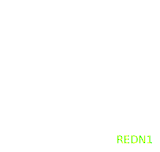
\includegraphics[align=c, width=0.48\textwidth]{Figures/ElectrodesExperimental/photo_redn1.jpg}
\includegraphics[align=c, width=0.48\textwidth]{Figures/ElectrodesExperimental/photo_red80.pdf}
\caption{Photos of the REDN1 detector (on the left) and the RED80 detector (on the right).}
\label{fig:photo-redn1-red80}
\end{figure}


\subsection{RED80 detector}

% Polarization
The detector RED80 has four electrodes:
\begin{itemize}
	\item the main collect electrodes $B$ and $D$, consisting of the top and bottom central planar pads respectively,
	\item the auxiliary guard electrodes $A$ and $C$, consisting of two top and bottom thin lateral rings respectively. 
\end{itemize}
Same-sided guard and collect electrodes have the same electric potential. The polarization of the detector can therefore be fixed with two parameters such that:
\begin{equation}
\begin{array}{cc}
V_A = V_B = & V_{bias} * S_{bias} \\
V_C = V_D = & - V_{bias} * \left( 1 - S_{bias} \right)
\end{array}
\end{equation}
with $V_{bias}$ the bias voltage and $S_{bias}$ the polarization symmetry parameter chosen in the interval $\left[ -1, 1 \right]$.

% Capacitance
The Maxwell capacitance matrix of the simulated detector RED80 is:
\begin{equation}
\bm{C} = 
\begin{pmatrix}
  13.93 & -6.32 & -3.89 & -2.57\\
  -6.32 & 17.17 & -1.91 & -6.06\\
  -3.89 & -1.91 & 14.25 & -7.28\\
  -2.57 & -6.06 & -7.28 & 18.61\\
\end{pmatrix}
\cdot \SI{e-12}{\farad}
\end{equation}

% Fiducial Volume
The theoretical fiducial volume percentage is estimated at $\%_{fid}=\SI{80.75}{\percent}$. The percentage of the volume attributed to other regions is less precise due to the limitation of the estimation technique ($z=0$). We estimate that $\%_{guard} \approx \SI{13}{\percent}$ and $\%_{corners} \approx \SI{5}{\percent}$.

\begin{table}[]
\centering
%\resizebox{\textwidth}{!}{%
\begin{tabular}{l c S}
Parameter                                   & Symbol        & {Default Value} \\ \hline \hline
Ge crystal Height                           & $H_{Ge}$      & \SI{10}{\mm}  \\
Ge crystal Radius                           & $R_{Ge}$      & \SI{15}{\mm}    \\
Distance between crystal and copper chassis & $d_{Cu}$      & \SI{3}{\mm}     \\
Aluminium Deposit Thickness                         & $h_{Al}$      & \SI{1}{\micro\meter}   \\
Width of the Lateral Rings                      & $w_{Al}$      & \SI{80}{\micro\meter}  \\
Radius of the Planar Electrode Pad  & $r_{center}$   & \SI{13.5}{\mm}   \\
Width of bare Ge crystal on edge     & $w_{bare}$    & \SI{1.5}{\mm}  \\
Spacing between Lateral Rings          & $d_{lat}$  & \SI{2.4}{\mm}  \\
Equatorial distance						& $d_{eq}$	& \SI{1.2}{\mm} \\
Offset on Equator Height				& $z_{eq}$	& \SI{-0.5}{\mm} \\
Main Voltage Bias                           & $V_{bias}$    & \SI{2}{\volt}      \\
Symmetric factor of the voltage bias        & $S_{bias}$    & {$0.5$}         
\end{tabular}
%}%
\caption{Parameter values for the default operation of the RED80 detector.}
\label{tab:red80-default-parameters}
\end{table}


\begin{figure}
\centering
\includegraphics[scale=1]{Figures/ElectrodesExperimental/scheme_red80.pdf}
\caption{Scheme of the RED80 detector.}
\label{fig:red80-scheme}
\end{figure}

\begin{figure}
\centering
\includegraphics[scale=0.5]{Figures/ElectrodesExperimental/potential_red80.png}
\includegraphics[scale=0.5]{Figures/ElectrodesExperimental/twp_red80.png}
\caption{Potential and TWP field of RED80.}
\label{fig:efield-red80}
\end{figure}

\begin{figure}
\centering
\includegraphics[align=c, scale=0.5]{Figures/ElectrodesExperimental/efield_red80.png}
\includegraphics[align=c, scale=0.5]{Figures/ElectrodesExperimental/enorm_hist_red80.pdf}
\caption{Electric field magnitude color map and Histogram of the magnitude distribution over the crystal volume of RED80.}
\label{fig:efield-red80}
\end{figure}


\subsection{REDN1 detector}

% Polarization
The detector REDN1 has four electrodes like the FID38 design. The main top and bottom collect electrodes are $B$ and $D$ respectively. The auxiliary top and bottom veto electrodes are $A$ and $C$ respectively. Each electrode is composed of multiples aluminium rings deposited on the planar surface of the crystal. In the same manner as the FID38, same-sided veto and collect electrodes are interleaved as according to the scheme \ref{fig:redn1-scheme}. Moreover, the polarization of the electrodes are the same as FID38 described in equation \ref{eq:fid-polarization}. The electric potential of the four electrodes $V_A, V_B, V_C, V_D$ are fixed by the same three parameters: the bias voltage $V_{bias}$, the polarization symmetry $S_{bias}$ and the polarization ratio $R_{veto}$. As such, in operation, the electric field in REDN1 forms the same volume in respect to the charge collection as the FID38 as illustrated by the colored regions in scheme \ref{fig:redn1-scheme}. With a particle recoil ionizing the medium in the bulk volume, the top veto volume or the bottom veto volume, the drifting electric charges induce the same signal as in the case of the FID38 design. The topology of the detector REDN1 only differs from the FID38 design by not having rings on the lateral surface of the crystal. As a result, the electric field lines cannot connect to the veto electrodes directly. The figure \ref{fig:efield-redn1} shows that the equatorial field lines rather exit the crystal in the vicinity of the equator, and only in the vacuum rejoin the edge veto electrodes. Assuming the electric charges exactly follows the electric field lines, all charges should be trapped on the lateral surface of the crystal. As the discussed in the paragraph ref{par:shockley-ramo}, the signal induced on the electrodes depends on their weighting potentials at the end of the charge drift, in this case the equatorial surface.
$$ Calculation ? $$
As the equatorial volume is small compared to the variation scale of the weighting potential field, we can consider the signal induced by electric charges to be null (rough approximation, we should have like \SI{10}{\percent} of the signal I think).

% Capacitance
The Maxwell capacitance matrix of the simulated detector REDN1 is:
\begin{equation}
\bm{C} = 
\begin{pmatrix}
  19.46 & -11.84 & -3.00 & -1.89\\
  -11.84 & 16.17 & -1.89 & -1.26\\
  -3.00 & -1.89 & 19.46 & -11.84\\
  -1.89 & -1.26 & -11.84 & 16.17\\
\end{pmatrix}
\cdot \SI{e-12}{\farad}
\end{equation}

\begin{table}[]
\centering
%\resizebox{\textwidth}{!}{%
\begin{tabular}{l c S}
Parameter                                   & Symbol        & {Default Value} \\ \hline \hline
Ge crystal Height                           & $H_{Ge}$      & \SI{10}{\mm}  \\
Ge crystal Radius                           & $R_{Ge}$      & \SI{15}{\mm}    \\
Distance between crystal and copper chassis & $d_{Cu}$      & \SI{3}{\mm}     \\
Electrode Thickness                         & $h_{Al}$      & \SI{1}{\micro\meter}   \\
Electrode Width                             & $w_{Al}$      & \SI{80}{\micro\meter}  \\
Radius of the innermost planar electrode    & $r_{center}$   & \SI{1.5}{\mm}   \\
Width of bare Ge crystal on corners      & $w_{bare}$    & \SI{0}{\mm}  \\
Width of the outermost veto electrode    & $w_{outer}$    & \SI{1}{\mm}  \\
Number of planar electrodes                 & $n_{plan}$  & {$9$}             \\
Interdistance of Planar electrodes          & $d_{plan}$  & \SI{1.5625}{\mm}  \\
Main Voltage Bias                           & $V_{bias}$    & \SI{2}{\volt}      \\
Ratio Veto/Main voltage bias                & $R_{veto}$    & {$0.375$}         \\
Symmetric factor of the voltage bias        & $S_{bias}$    & {$0.5$}         
\end{tabular}
%}%
\caption{Parameter values for the default operation of the REDN1 detector.}
\label{tab:redn1-default-parameters}
\end{table}

\begin{figure}
\centering
\includegraphics[scale=1]{Figures/ElectrodesExperimental/scheme_redn1.pdf}
\caption{Scheme of the REDN1 detector.}
\label{fig:redn1-scheme}
\end{figure}

\begin{figure}
\centering
\includegraphics[scale=0.5]{Figures/ElectrodesExperimental/potential_redn1.png}
\includegraphics[scale=0.5]{Figures/ElectrodesExperimental/twp_redn1.png}
\caption{Potential and TWP field of redn1.}
\label{fig:efield-redn1}
\end{figure}

\begin{figure}
\centering
\includegraphics[align=c, scale=0.5]{Figures/ElectrodesExperimental/efield_redn1.png}
\includegraphics[align=c, scale=0.5]{Figures/ElectrodesExperimental/enorm_hist_redn1.pdf}
\caption{Electric field magnitude color map and Histogram of the magnitude distribution over the crystal volume of redn1.}
\label{fig:efield-redn1}
\end{figure}

\begin{figure}
\centering
\includegraphics[scale=1]{Figures/ElectrodesExperimental/redn1_experimental_fiducial_volume.pdf}
\caption{Experimental Fiducial volume for REDN1.}
\label{fig:redn1-experimental-fiducial-volume}
\end{figure}



\section{Analysis Pipeline}


\section{Experimental Setup}

{\color{red} Two subsections: RED80 detector (describing RED80, sensitivity, electric field, polarization), Operation in cryostat (describing the temperature, the suspended tower, the configuration Calibration and Background, the calendar of the streams)}

The measurement of the neutron background at the IP2I cryogenic facility was done with a newly designed low-threshold germanium detector of the RED series called RED80 with RMS resolution of approximately 120eV on the heat channel and 200eV on the ionization channel.
The data were taken during the run 57 which began on 03/07/2019 and ended on 01/08/2019. In this run, RED80 and RED70 were both operated on the suspended tower.

\begin{figure}
\centering
\begin{subfigure}{.5\textwidth}
  \centering
  \includegraphics[width=\linewidth]{Figures/Neutron/photo_red80.png}
  \caption{Photo of RED80}
  \label{fig:photo-red80}
\end{subfigure}%
\begin{subfigure}{0.5\textwidth}
  \centering
  \includegraphics[width=\linewidth]{Figures/Neutron/scheme_red80.png}
  \caption{Scheme of RED80}
  \label{fig:scheme-red80}
\end{subfigure}
\caption{Description of RED80, with a schematic drawing of the Germanium crystal, the NTD sensor and the position and polarization of the electrodes.}
\label{fig:description-red80}
\end{figure}

% Description of RED80
RED80 is composed of a 38g cylindrical germanium crystal of height 10mm and diameter 30mm.
It is equipped with a heat channel and an ionization channel (see figure \ref{fig:description-red80})
The ionization channel consists of a pair of collecting electrodes and guard electrodes.
The collecting electrodes are two flat full aluminium electrodes of diameter 27mm deposited on its top and bottom surface.
The guard electrodes are four circular electrodes deposited on its side.
The heat channel consists of a NTDGe thermistance labeled K58 with dimension 4*4*0.45 mm.
Before being installed into the cryostat, the detector was place near a neutron source in order to activate the Germanium crystal and benefit from the intrinsic gamma calibration peak during operation. The neutron activation started on 28/06/2019 at 17h08 and ended on 02/08/2019 at 10h08 yielding 89h of activation.

% Conditions of data taking
From 08/08/2019, the detectors were characterized at 18mK. As for the actual condition of the neutron background measuremets, RED80 was operated at 16mK with an optimal NTD polarization current of 1nA and an electric potential difference of 2V on the ionization channel:
$$ A, B, C, D = +1, +1, -1, -1.$$

The data taking was divided between two configurations, "Background" and "Calibration", meant to measure the neutron background and calibrate the neutron recoil band in the detector respectively.
The Background configuration was used to save 34 hours of data partitioned in three streams: tg18l005, tg27l000 and tg28l000.
The Calibration configurations was used to take 78 hours of data, with an Americium-Beryllium neutron source situated 4.5m away from the cryostat and shielded with milk (acting as water) to thermalize the emitted neutron (see figure ??). The data were saved in four streams: tg17l007, tg19l010, tg20l000 and tg21l000.

\begin{figure}
\centering
\begin{subfigure}{.5\textwidth}
  \centering
  \includegraphics[width=\linewidth]{Figures/Neutron/photo_source_front.jpg}
  \caption{Front view, towards the cryostat}
  \label{fig:photo-source-frontt}
\end{subfigure}%
\begin{subfigure}{0.5\textwidth}
  \centering
  \includegraphics[width=\linewidth, angle=-90]{Figures/Neutron/photo_source_rear.jpg}
  \caption{Rear view}
  \label{fig:photo-source-rear}
\end{subfigure}
\caption{Photo of the shielded AmBe neutron source used for the neutron calibration.}
\label{fig:photo-source}
\end{figure}

Each stream was taken during nights or week-ends to benefit from the long time with stable operation (see Table \ref{tab:neutron-streams}). The configurations were mixed in term of dates, which is of importance when measuring the rate of the Germanium calibration peaks which is decreasing with time.

\begin{table}[]
\centering
\begin{tabular}{l|l|r}
Configuration                & Stream   & Started at          \\ \hline
\multirow{3}{*}{Background}  & tg18l005 & ?? on 18/08/2019    \\
                             & tg27l000 & 21h20 on 27/08/2019 \\
                             & tg28l000 & 11h27 on 28/08/2019 \\ \hline
\multirow{4}{*}{Calibration} & tg17l007 & ?? on 17/08/2019    \\
                             & tg19l010 & 17h10 on 19/08/2019 \\
                             & tg20l000 & ?? on 20/08/2019    \\
                             & tg21l000 & ?? on 21/08/2019   
\end{tabular}
\caption{Starting hours and date of the streams for neutron background and calibration measurements.}
\label{tab:neutron-streams}
\end{table}


\section{Pre-processing and Data format}
\label{par:data-format}
\label{par:of-processing}

The data were initially saved as streams: the voltage value of the heat channel and the four ionization channel are saved for each time step in the acquisition with a sampling frequency of 400Hz. 

\begin{figure}
\centering
\includegraphics[width=\linewidth,]{Figures/Neutron/event_example.png}
\caption{Raw signals in ADU of a triggering event.}
\label{fig:event-example}
\end{figure}

These voltage values are extracted by an analog-to-digital conversion system and thus expressed in \textbf{A}nalog-to-\textbf{D}igital conversion \textbf{U}nit (ADU).
These data streams are then processed by an \textbf{O}ptimal \textbf{F}iltering (OF) software called NEPAL. A filter based on the signal PSD and the noise PSD in the bolometer is applied to the stream. Time windows of 1s centered on a triggering events are selected with an amplitude threshold on the filtered stream (see Figure \ref{fig:pulse-of}).

\begin{figure}
\centering
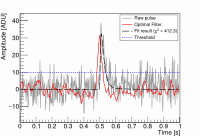
\includegraphics[width=\linewidth,]{Figures/Neutron/pulse_of.png}
\caption{Optimal filtering of a 1s pulse window.}
\label{fig:pulse-of}
\end{figure}

These time windows are processed to extract several quantities:
\begin{itemize}
	\item Timestamp,
	\item Amplitude (filtered decorrelated),
	\item Chi2 value (filtered decorrelated),
	\item Offset (raw),
	\item Ionization Slope (raw),
\end{itemize}
The figure \ref{fig:analysis-monitoring-demo} shows this characterization quantities for each triggering event as a function of their timestamp (for the considered stream, here tg17l007). Each scatter plots is understood when applying the quality cut:
\begin{itemize}
	\item Heat Energy vs Timestamp: Reconstruction of the energy deposited in the heat channel for each event. This graph can be linked to the heat energy spectrum presented later. One can note pronounced population of fixed energy corresponding to the abundance of 10.37keV events due to the activation of the Germanium crystal and the noise blob poulation at $\mathcal{O}(50)$eV.
	\item Ionization Energy vs Timestamp: is quite the same as heat energy, except that with the overlap of the different channels this graph is now an useless mess
	\item Offset Heat vs Timestamp: this curve is proportional to the resistance value of the NTD sensor and allows us to follow the baseline temperature. With this decreasing profile, we deduce that the detector has been cooling during this stream. Note that although RED80 is still slowly thermalizing, the sensitivity is stable (precision?)
	\item Offset Ionization vs Timestamp: this curve is essentially used to discard all the events with an offset outside of the $[-14000, 14000]$ ADU (see \ref{par:quality-cuts}).
	\item Slope Ionization vs Timestamp: this curve is proportional to the baseline current measured by each electrodes. This baseline current is explained by the presence of leakage current between the electrodes (dedicated section?) and the collection of trapped charges (especially after a maintenance).
	\item Chi2 vs Timestamp: This describes the goodness of the fit of the template to the pulse. A stable low value indicate a fixed shape for the pulses, which is required for the chi2 cut applied later (see \ref{par:quality-cuts})
\end{itemize}

\begin{figure}
\centering
\includegraphics[width=\linewidth,]{Figures/Neutron/analysis_monitoring_demo.png}
\caption{Characterization quantities of triggering events as a function of their timestamp. (TO BE CHANGE !)}
\label{fig:analysis-monitoring-demo}
\end{figure}

In the end, for each configuration of data measurements(Background and Calibration), triggering events were selected in each streams and described by several quantities.
Among those triggering events are events of interest well reconstructed and induced by electronic recoil from the radioactive gamma background, the KLM activation lines from the germanium and the cosmic muons and neutron recoil from the AmBe neutron source and the radioactive neutron background. However, many triggering events can not be reconstructed or were induced by parasitic source, and can not yield information for the measurement of the neutron background at IP2I. To extract the events of interest from all the data, analysis cuts are applied.


\section{Quality Cuts}
\label{par:quality-cuts}

The objective of the "Quality cut" is to keep the events induced by recoils in the germanium absorber of RED80 and with a good energy reconstruction. These events  passing the Quality cut are labeled as "quality events" and satisfy several criteria:
\begin{itemize}
	\item passing the Livetime Cut,
	\item not happening during a maintenance period of the ionization channel,
	\item offset of the ionization channel in the $[-14000, +14000] ADU$ interval,
	\item the $\chi^2$ value, expressing the goodness of the fit of the event with the signal template.
\end{itemize}

{\color{red} Maintenance cut paragraph, will surely be moved in the section describing the electronics.}
\label{par:reset-maintenance}
The electrodes of the ionization channel are collecting the electron-hole pairs induced by the recoils in the germanium crystal. As a results, their electric potential is decreasing (recall $Q=CU$) as well as the electric field guiding the e-h pairs in the crystal. In order to keep a steady electric field, it is necessary to periodically recharge the electrodes, offsetting the effect of the e-h pairs collection. This process is called "Reset" and is usually set to happen every few seconds in detectors.
An adverse effect of these resets is that they usually induce a signal on the heat and ionization channels. While these signals are easily discarded using their known frequency, they can happen close to a valid signal resulting in a pile-up, the discarding of the event from the analysis, and so a decrease in the livetime of a data stream.

Another phenomenon degrading the electric field is the trapping of the charges in the crystal. Even if the electrodes are properly "resetted", the accumulating trapped charges produces a counter-field effectively reducing the electric field seen by the e-h pairs in the crystal. The method used to even the charges in the crystal is called "Maintenance". The electrodes are successively polarized at plus and minus their nominal electric potential with a frequency of $\mathcal{O}(1\textsf{Hz})$ for about a minute. The trapped charges are shaken up in the crystal and eventually recombine or are collected at the electrodes. The counter-field vanishes and the detector is ready to operate with its standard electric field (graph necessary to illustrate ?). A downside is that the detector is not available for data taking during a maintenance, representing about a minute of deadtime for several tenths of minutes of running time. 

As this work uses data taken with detectors operated in an above-ground laboratory, the event rate is higher compared to an underground facility due to the abundance of cosmic rays and the natural radioactivity.
With this higher event rate  comes a higher charge collected per unit of time. This induces a quicker decrease of the electric potential of the electrodes, which needs for more frequent resets, and a quicker appearing of the counter-field due to the charge trapping, which calls for more frequent maintenances.

Thus, the frequency of the reset and the maintenance is adapted to the event rate seen by the detectors. The reset and maintenance should be frequent enough to keep up with the electric field decrease, yet spaced out to keep a reasonable livetime. Moreover, the event rate do fluctuate between each run as it depends on the mass of the absorbers (here 32g, 38g or 200g) and the possible use of calibration sources increasing the event rate (see the section \ref{par:calibration-sources}).
In average in this work, the resets are set to a frequency of $2$Hz (?) and maintenance set to take place every 40 minutes.
{\color{red} End of Maintenance paragraph}

Quality events should not happen during a maintenance period nor a reset (introduced in section \ref{par:reset-maintenance} as they are considered electronics artifacts. The "Maintenance cut" is defined as:
$$ bli blou bloup$$
which discards any event happening during a maintenance period.
The "Reset cut" is expressed as:
$$ hello there general$$
which discards event occurring within $5$ms (?) of a reset. 
{\color{red} INSERT MATHEMATICAL DEFINITION of the maintenance cut and the reset cut. And implement it correctly in the analysis! }

{\color{red} paragraph about the ion sensitivity degradation past 14000ADU. Dont know if this is gonna stay in this chapter or move it when describing the electronics. Feel like it should belong here, as I can illustrate that with a figure}

We noticed a malfunction for the ionization channel: apparently, the sensitivity of the ionization channels depends on their offset value. This behavior is consider as faulty as we expect the electrodes to have a constant sensitivity. This phenomenon is illustrated in the figure \ref{fig:offset-problem} which plots the ionization amplitudes of events as a function of their offset values for the data stream "???".

\begin{figure}
\centering
\includegraphics[width=\linewidth, height=6cm]{Figures/Neutron/offset_cut.png}
\caption{Graph of the reconstructed amplitude of the triggering events on the ionization channel D in function of their offset value. The dense population of 10keV calibration events with a reconstructed ionization energy of about 60ADU let us monitor the sensitivity of the electrodes. We note that past 23000 ADU of offset, the electrodes becomes half as sensitive as before with the 10keV calibration population reconstructed at 30ADU. The red overlay span illustrates the region discarded by the offset cut.The data presented corresponds to the stream "tg18l005". }
\label{fig:offset-problem}
\end{figure}

INTERPRETATION when plot is ready.
We decide to keep the events with the standard ionization sensitivity with low absolute offset value. Other events are discarded by the "Offset cut" which is expressed as:
$$ mathemics here $$


Concerning the $\chi^2$ value, the threshold depends on the energy. Indeed, because of non-linearity in the bolometer heat response, the shape of the signal do depends on the recoil energy as the first order perturbation theory becomes less and less valid.
Good events at low energy should have a $\chi^2$ value of about:

\begin{equation}
\mathbb{E}\left( \chi^2 \right) 
= N_{\textsf{samples in window}}
 = T_{\textsf{window}} \times f_{\textsf{sampling}}
 = 0.5 \times 400 = 200
\end{equation}

However, with a signal template based on events from the 10.37keV activation line of the germanium, the $\chi^2$ value of good events is increasing from $\mathcal{O}(10keV)$.
Therefore, a cut parametrization function depending on the event amplitude is chosen:

\begin{equation}
Threshold(Amplitude) 
= \gamma \times \mathbb{E}\left( \chi^2 \right)  \times \left[ 1+ \left( \frac{Amplitude}{\alpha} \right)^\beta \right]
\end{equation}

with $\alpha$, $\beta$ and $\gamma$ estimated visually for each streams and presented in table \ref{tab:chi2-cut}.

\begin{table}[]
\centering
\begin{tabular}{l|l|l|l|l}
Channel type                & $\alpha$                         & $\beta$              & Streams              & $\gamma$           \\ \hline \hline
\multirow{7}{*}{Heat}       & \multirow{7}{*}{$2 \times 10^3$} & \multirow{7}{*}{2}   & tg17l007             & 1                  \\
 &  &  & tg18l005 & 1    \\
 &  &  & tg19l010 & 1    \\
 &  &  & tg20l000 & 1    \\
 &  &  & tg21l000 & 1    \\
 &  &  & tg27l000 & 1.75 \\
 &  &  & tg28l000 & 1.75 \\ \hline
\multirow{7}{*}{Ionization} & \multirow{7}{*}{$3 \times 10^2$} & \multirow{7}{*}{2.2} & \multirow{7}{*}{All} & \multirow{7}{*}{1} \\
 &  &  &          &      \\
 &  &  &          &      \\
 &  &  &          &      \\
 &  &  &          &      \\
 &  &  &          &      \\
 &  &  &          &     
\end{tabular}
\caption{Coefficient of the $chi^2$ cut for each streams. These coefficients were determined visually in order to defined the band of events of lowest $chi^2$ value on the whole energy range.}
\label{tab:chi2-cut}
\end{table}


In the end, the $\chi^2$ cut is applied on each channels (as seen in figure \ref{fig:chi2-cut}) independently. Only the events passing the cut for all the channels is kept and eligible as a quality event.

\begin{figure}
\centering
\includegraphics[width=\linewidth,]{Figures/Neutron/chi2_cut.png}
\caption{$\chi^2$ value for each event in function of its reconstructed amplitude for the five measuring channels. The cut threshold is represented by the black line. All events are in red, passing events are in blue.}
\label{fig:chi2-cut}
\end{figure}

With all these criteria being applied to the events passing the Livetime Cut, we have selected the events passing the Quality Cut, qualified as "quality events".



\subsection{Cross-talk correction and Cabling capacitance estimation}

With the selection of the fiducial events, it is possible to estimate precisely the cross-talk correction matrix and the cabling capacitance.

A fiducial recoil leads to an electric charge perturbation expresses by the vector $\vec{Q}$ such that:
\begin{equation}
\vec{Q}_{fid}^{REDN1} =
\begin{bmatrix}
0 \\ -1 \\ 0 \\ 1
\end{bmatrix}
\cdot Q(\SI{10.37}{\kilo\eV})
\end{equation}
with the electric charge multiplicative factor being:
\begin{equation}
Q(\SI{10.37}{\kilo\eV})
=
N_p(\SI{10.37}{\kilo\eV}) \cdot e
=
\frac{E_R}{\epsilon} e
=
\frac{\SI{10.37e3}{\eV}}{\SI{3}{\eV}} e
\end{equation}

According to equation \ref{eq:matrix-capacitance-charge}, the voltage signal induced on the electrodes is expressed by the vector $\vec{V}_{fid}^{REDN1}$ obtained with the Maxwell capacitance matrix  of the detector and cabling $\bm{C}_{total} = \bm{C}_{detector} + \bm{C}_{cabling}$ such that:
\begin{equation}
\label{eq:redn1-bulk-voltage-vector}
\vec{V}_{fid}^{REDN1}
=
\begin{bmatrix}
V_A \\ V_B \\ V_C \\ V_D
\end{bmatrix}
=
\bm{C}_{total}
\cdot
\vec{Q}_{fid}^{REDN1}
\end{equation}

In the paragraph \ref{par:sensitivity-calculation}, the Maxwell capacitance matrix associated with the cabling $\bm{C}_{cabling}$ is considered to be diagonal with $\forall i \neq j, \bm{C}_{cabling, ij} = 0$ . The previous equation \ref{eq:redn1-bulk-voltage-vector} can be translated for the terms $\bm{V}_{i}$ and $\bm{Q}_i$ of the vectors $\vec{V}_{fid}^{REDN1}=\vec{V}$ and $\vec{Q}_{fid}^{REDN1}=\vec{Q}$ respectively:
\begin{equation}
\bm{V}_{i}
=
\sum_{j=1}^4 \bm{C}_{total, ij} \bm{Q}_j
=
\sum_{j=1}^4 \bm{C}_{detector, ij} \bm{Q}_j + \sum_{j=1}^4 \bm{C}_{cabling, ij} \bm{Q}_j
=
\left( \bm{C}_{detector, i4} - \bm{C}_{detector, i2} \right) Q(\SI{10.37}{\kilo\eV}) + \bm{C}_{cabling, ii} \bm{Q}_i
\end{equation}

We assume that the Maxwell capacitance matrix relative to the detector $\bm{C}_{detector}$ is known as it calculated from the electrostatics simulation of REDN1. The diagonal terms $\bm{C}_{cabling, ii}$ of the cabling capacitance matrix can therefore be evaluated from the voltage signal induced by the \SI{10.37}{\kilo\eV} fiducial events $\bm{V}_{i}$ :
\begin{equation}
\label{eq:cabling-capacitance-expression}
\bm{C}_{cabling, ii}
=
\frac{1}{\bm{Q}_i} \left[ \bm{V}_{i} - \left( \bm{C}_{detector, i4} - \bm{C}_{detector, i2} \right) Q(\SI{10.37}{\kilo\eV}) \right]
\end{equation}

One should note that as $\bm{Q}_1 = \bm{Q}_3 = 0$, the equation \ref{eq:cabling-capacitance-expression} is only valid for $i \in \{ 2,4 \}$. This means that the fiducial events collected by the electrode $B$ and $D$ can only be used to determine the cabling capacitance associated with these very electrodes $\bm{C}_{cabling, 22}$ and $\bm{C}_{cabling, 44}$ respectively.


\underline{FROM CHAPTER NEUTRON} 

While the heat channel can readily be calibrated, this is not the case for the ionization channel which are affected by a phenomenon of cross-talk which should be corrected before proceeding with their calibration.
Because of the capacitive coupling between the different electrodes of the bolometer, a signal collected by an electrode will induce another smaller signal on other electrodes. With such a coupling, the cross-talk factor between two electrodes increases with their associated capacitance term.
As a result, for a small bolometer as RED80 with capacitance terms in $\mathcal(O)(10 pF)$, the cross-talk factors are about few percents. This is to be compared to the bigger 200g FID bolometers used in EDELWEISS-III, with an increased capacitance of $\mathcal(O)(100 pF)$, presenting cross-talk factors of about few tens of percent.
The real ionization channels $A,B,C,D$ affected by the crosstalk can be corrected into decoupled ionization channels $A', B', C', D'$ according to the following equation:

\begin{equation}
	\left[\begin{array}{c}
	A' \\ 
	B' \\ 
	C' \\ 
	D'
	\end{array}\right]
	=
	\mathcal{M}
	\left[\begin{array}{c}
	A \\ 
	B \\ 
	C \\ 
	D
	\end{array} \right]
\end{equation}
with $\mathcal{M}$ the cross-talk correction matrix being:
\begin{equation}
	\mathcal{M}
	=
	\left[\begin{array}{cccc}
	1 & -0.052 & 0 & 0 \\ 
	-0.03 & 1 & 0 & 0 \\ 
	-0.012 & 0.001 & 1 & -0.025 \\ 
	0 & 0 & -0.03 & 1
	\end{array}\right]
\end{equation}

The terms of this correction matrix were found with the study of specific populations of events of known characteristics (as seen in figure \ref{fig:scheme-red80}):
\begin{itemize}
	\item Bulk events are collected by the main electrodes and no charge is collected by the guard electrodes with $$A'= C' = 0$$
	\item Surface events are collected by the guard electrodes and no charge is collected by the main electrodes with $$B' = D' = 0$$
\end{itemize}

This correction is implemented iteratively by visually checking the plotting of the corrected ionization channels against themselves. The figure \ref{fig:crosstalk-correction} shows the signals of the events of the uncorrected ionization channels $A, B, C, D$ as black points. Superposing to this are the blue points associated with the events of the decoupled ionization channels $A', B', C', D'$.

\begin{figure}
\centering
\includegraphics[width=\linewidth,]{Figures/Neutron/crosstalk_correction.png}
\caption{Corner plot of the reconstructed ionization energies of the quality events. Energies affected by the cross-talk are in grey/black, corrected energies are in blue. The x-axis and y-axis are plotted in red as visual guides.}
\label{fig:crosstalk-correction}
\end{figure}

We check that the cross-talk correction matrix $\mathcal{M}$ corresponds to the identity matrix at the first order. The correction terms are in the range of few percents, going up to $5.2\%$ in the case of the case of the electrode $B$ inducing signal on the electrode $A$.


\begin{figure}
\centering
\includegraphics[scale=1]{Figures/ElectrodesExperimental/redn1_cabling_capacitance_fitting.pdf}
\caption{Fitting the cabling capacitance for REDN1.}
\label{fig:red80-cabling-capacitance}
\end{figure}


\begin{figure}
\centering
\includegraphics[scale=1]{Figures/ElectrodesExperimental/red80_cabling_capacitance_fitting.pdf}
\caption{Fitting the cabling capacitance for RED80.}
\label{fig:red80-cabling-capacitance}
\end{figure}


\section{Calibration}
\label{par:calibration}

The five measurements channels are saving the voltage of their associated sensors in ADU unit specific to each considered channel. In order to proceed with physical interpretation, it is now necessary to convert the channels into a common unit.
For this purpose, we use the activation of the KLM lines of the Germanium crystal, which emits a gamma of energy 100eV, 1.3keV and 10.37keV respectively [\cite{germanium-decay}]. This gammas of known energy produce electronic recoils depositing a known energy in the ionization channels and the heat channel, with the latter being boosted with the Luke-Neganov effect [\cite{luke-neganov-effect} and \citep{luke-neganov-interpretation}]. As the quenching of the electronic recoil is different from the one of the nuclear recoil, we use the $keV_{ee}$ which precise that the energy deposit done with an electronic recoil.

Concerning the ionization channels, we use the 10.37keV line forming a multivariate normal distributed blob in the figure \ref{fig:calibration-ion} showing the signal of an event in each ionization channel in ADU unit. We estimate the center of this distribution to be $55$ ADU for each channels. We can now deduce the calibration coefficient for the ionization channels : $\pm 55 ADU \leftrightarrow 10.37 keV_{ee}$.

\begin{figure}
\centering
\includegraphics[width=\linewidth,]{Figures/Neutron/calibration_ion.png}
\caption{Corner plot of the reconstructed ionization amplitude of the quality events, zoomed on the 10.37keV calibration peak.}
\label{fig:calibration-ion}
\end{figure}

As for the heat channel, we use the 10.37keV line forming a normal distribution visible in the ADU amplitude spectrum of the heat channel as seen in figure \ref{fig:calibration-heat}. The estimated center of this distribution is $1200$ ADU. The calibration coefficient for the heat channel is therefore: $1200 ADU \leftrightarrow 10.37 keV_{ee}$.

\begin{figure}
\centering
\includegraphics[width=\linewidth,]{Figures/Neutron/calibration_heat.png}
\caption{Heat Amplitude Spectrum for a stream. The calibration coefficient is estimated from the 10.37keV calibration peak position.}
\label{fig:calibration-heat}
\end{figure}

With these calibration coefficient, it is now possible to reason with the reconstructed energy for each channels as
$$
\textsf{Reconstructed energy [keV]}
=
\textsf{Calibration Coefficient [keV/ADU]}
\times
\textsf{Event Amplitude [ADU]}
$$
Now that the events of all the streams are calibrated, they are expressed in the same unit and can be compared. From now on, we concatenate the calibrated streams and consider all the events for the Background and the Calibration configurations.


\section{Charge conservation cut}
\label{par:charge-conservation-cut}

to be corrected vvv
Even with the bulk cut, some events might still have charge collection issue. Drifting charges can be trapped in the germanium and may not end up being collected. On way to discard such events is to consider the "Charge Conservation" quantity, defined as:
\begin{equation}
\mathcal{C.C.} = \frac{-A-B+C+D}{2}
\end{equation}

As a recoil produces electron-hole pairs, the charge of the drifting particles in the crystal should be zero as well as the total collected charges (considering their complete collection). This is characterized by a the normal distribution of the $\mathcal{C.C}$ around zero with an STD depending on the RMS resolution of the ionization channels. Events with an incomplete charge collection would stand out of this gaussian profile and can be discarded. As a result, we define the event passing this "Charge conservation cut" with a $\mathcal{C.C.}$ lower than two times the RMS resolution for the considered heat energy. This cut is represented in the figure \ref{fig:charge-conservation}.

\begin{figure}
\centering
\includegraphics[width=\linewidth,]{Figures/Neutron/charge_conservation.png}
\caption{"Charge conservation" quantity as a function of the heat energy for the bulk quality events of the Background configuration. Passing events are in blue while discarded events are in red.}
\label{fig:charge-conservation}
\end{figure}

As the RMS resolution depends on the energy associated to the event, it is once more necessary to model it with a linear law:
\begin{equation}
\sigma_{\mathcal{C.C.}}\left(E_{heat}\right)
=
a + b*E_{heat}
\end{equation}
with the coefficient $a$ and $b$ coming from the estimation of the RMS resolution at 0keV (noise blob) and 10.37keV (calibration peak) (precision necessary here).


\subsection{Fiducial Cut}
\label{par:fiducial-cut}

Referring to the streamlines of the electric field in the crystal of RED80 (see Figure \ref{fig:streamlines-red80}), we expect some region of the crystal with a specific drifting behavior. Represented in the Figure \ref{fig:scheme-red80}, we have:
\begin{itemize}
	\item the Bulk region, where the charge will drift towards the collect electrodes B and D,
	\item the Guard region, where the charge will be collected by the surface electrodes A and C,
	\item the Corner regions, where and , we expect the charges to recombine on place of the recoil because of the very weak electric field or become trapped on the surface by drifting along the streamlines exiting the crystal.
\end{itemize}

Surface regions are always hazardous for charge collection. Indeed, EDELWEISS has a knowledge (ref necessary) of charges drifting close to the surface devoid of electrodes being easily trapped and not being collected. This behavior is degrading the ionization signal leading to a recoil with reduced quenching factor. This means that electronic recoils happening near the surface could be reconstructed with a lower quenching and be identified as nuclear recoils. The major source of such surface recoil are the $\beta$ radiation induced by the natural radioactivity interacting in the first $\mu$m of the germanium crystal (ref edelweiss necessary). Thus, we want to discard any event that may be induced by a surface recoil. When interacting on the lateral surface of the germanium crystal, this events should be collected by the guard electrodes A and C. Referring to the scheme \ref{fig:scheme-red80}, the objective of the "Fiducial cut" is to discard events from the Surface zones and Corners, and keep the events induced by recoil in the bulk region of the crystal. This Fiducial cut is applied by considering the reconstructed ionization energy of the events as represented in the figure \ref{fig:fiducial-cut}.

\begin{figure}
\centering
\includegraphics[width=\linewidth,]{Figures/Neutron/fid_cut.png}
\caption{Corner plot of the reconstructed ionization energy for each electrodes for the quality events of the Background configurations. The energy thresholds for the cuts as well as the passing events are highlighted in the associated colors: blue for "bulk cut" and red for "guard cut".}
\label{fig:fiducial-cut}
\end{figure}

The Fiducial cut identifies events of the bulk region as events which did not deposited any signal on the guard electrodes A and C, with a tolerance of two $\sigma^{A,C}\left( \textsf{baseline} \right)$. For the bulk events, this conditions is expressed as:

\begin{equation}
mathmathmath for bulk events
\end{equation}

In a similar manner, we can also define the guard events with no signal on the collect electrodes B and D with a tolerance of two $\sigma^{B,D}\left( \textsf{baseline} \right)$. This condition then is written:

\begin{equation}
mathmathmath for guard events
\end{equation}

{\color{red}NOW, ITS GIBBERISH TIME !(yay, but to be modified)}
This "Bulk cut" will discard any event with a reconstructed energy on the guard electrodes A and C which is greater than two times the RMS resolution.
For this purpose, it is useful to define the reconstructed total ionization energy:
\begin{equation}
E_{ion., total} = \frac{A+B+C+D}{2}
\end{equation}

%\begin{itemize}
%	\item Ionization Energy in the Bulk region: $E_{ion., bulk} = \frac{B+D}{2}$
%	\item Ionization Energy in the Guard region: $E_{ion., guard} = \frac{A+C}{2}$
%	\item Total Ionization Energy: $E_{ion., total} = \frac{A+B+C+D}{2}$
%\end{itemize}

As the RMS resolution $\sigma_i$ of given channel $i$ depends on the total ionization energy deposited in the crystal, it is modeled by a power law:
\begin{equation}
\sigma_i\left( E_{i, total} \right)
=
\sqrt{ 
\left( \sigma_i(0\textsf{keV}) \right)^2 + 
\left( \alpha E_{ion., total} \right)^2
}
\quad \textsf{with} \quad
\alpha = \frac{\sqrt{\sigma_i(10.37\textsf{keV})^2 - \sigma_i(0\textsf{keV})^2}}{10.37 \textsf{keV}}
\end{equation}
In this equation, the baseline resolution $\sigma_i(0\textsf{keV})$ is estimated with the standard deviation of the noise blob while the resolution $\sigma_i(10.37\textsf{keV})$ is estimated with the standard deviation of the events associated to the germanium calibration peak.
{\color{red}END of GIBBERISH, i think}


%\subsection{Review of the selected events}

We have discarded the events with a possible bad energy reconstruction energy and calibrated the remaining ones. The experimental signal obtained with the heat and ionization channels were reconstructed into heat energy $E_{heat}$ and total ionization energy $E_{ion.}$. The figure \ref{ecei-plot} shows the scatter plot of these two values for the events of the Calibration configuration.

\begin{figure}
\centering
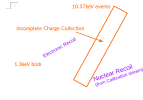
\includegraphics[width=\linewidth,]{Figures/Neutron/ecei_plot.png}
\caption{Reconstructed Ionization Energy in function of the Reconstructed Heat Energy, for the quality events of the Calibration configuration. The plot is zoomed up to 12keV for an easier view of the calibration peaks. }
\label{fig:ecei-plot}
\end{figure}

We recognize the noise blob near the origin corresponding to recoils of very low energy and triggering noise windows. Expanding from this noise blob, we note two bands. 
The electronic recoil band corresponds to events depositing the same energy in the ionization channel and the heat energy channel (both in keVee). They are characterized by a quenching factor of 1. As a matter of fact, the gamma recoil of 1.3keV and 10.37keV coming from the calibration peaks of the germanium belongs to this band. Any event below this band deposited less energy in the ionization channel than in the heat channel, and therefore possess a quenching factor inferior to one. We see that the population blob associated to the 10.37keV is smeared to lower quenching factor. This is due to events of the calibration peaks with incomplete charge collection. We note that this population is following a linear trend, which can be explained by an incomplete Luke-Neganov Boost of the heat channel according to the equation:
\begin{equation}
E_{heat} = 6 \textsf{keVee} + \epsilon \frac{2 \textsf{V}}{\epsilon_{Ge}} E_{ion.}
\end{equation}
The other major population of events below the electronic recoil band counts a lot of events in the case of the Calibration configuration. This hints that this band corresponds to the nuclear recoil induced by the AmBe neutron source.
The presence of the two bands in this plot demonstrate the discriminating ability of the associated heat and ionization channels. Note that, although the bands are well separated at high energy, they are merging at low energy due to their width which is fixed by the energy resolution of the heat and ionization channel.

Another way to represent the discrimination between the electronic and the nuclear recoil is to compute the recoil energy $E_R$ and the quenching factor $Q$ for each event:
\begin{align}
\label{eq:quenching-from-ecei}
	E_{NL} &= \frac{V}{\epsilon} ( E_{ion., ???} - E_{heat} )
	\\
	E_R = E_{heat} - E_{NL} &= E_{heat} \left( 1 + \frac{V}{\epsilon} \right) - E_{ion., ???} \frac{V}{\epsilon}
	\\
	Q &= \frac{E_{ion., ???}}{E_R}
\end{align}
with $E_{NL}$ being the heat energy boost coming from the Neganov-Luke effect \cite{luke-neganov-effect}.
The recoil energy $E_R$ is expressed in the usual $keV$ energy unit, as the Luke-Neganov Boost depending on the type of recoil was substracted from the heat energy. The Quenching factor is unitless.
The figure \ref{fig:quenching_plot} show, for each configuration, the quenching factor as a function of the recoil energy.

\begin{figure}
\centering
\includegraphics[width=\linewidth,]{Figures/Neutron/quenching_plot.png}
\caption{Quenching value $Q$ for each quality events of the Background (black) and Calibration (blue) configurations in function of their recoil energy $E_R$.}
\label{fig:quenching_plot}
\end{figure}

We recognize the electronic band, centered around $Q=1$ and the nuclear recoil band with $Q<0.4$. We also note some inter-band events like the smearing of the 10.37keV events hinting at the incomplete charge collection.

%HEAT ONLY EVENT
However, there are some interesting events with a quenching factor $Q=0$ which are known as "Heat-only" events. This population is infamously known in domains in the EDELWEISS experiment [ref?] and CRESST [ref?]. This population could correspond to events with no charge collection, but this is not compatible with the lower count of inter-band events with an incomplete charge collection. An other and more realistic explanation would be the existence of energy deposit in the crystal without ionization. The source of this Heat-only event is still under investigation [ref?].

The merging phenomenon of the bands at low energy is also more visible in this graph with the change of variable. We can even visually witness that the lower part of the 1.3keV event blob is leaking into the higher part of the nuclear band.


\subsection{Experimental Estimation of the Fiducial Volume}


\subsubsection{RED80}

\begin{figure}
\centering
\includegraphics[scale=1]{Figures/ElectrodesExperimental/red80_experimental_fiducial_volume.pdf}
\caption{Experimental Fiducial volume for RED80.}
\label{fig:redn1-experimental-fiducial-volume}
\end{figure}


\subsubsection{REDN1}

\begin{figure}
\centering
\includegraphics[scale=1]{Figures/ElectrodesExperimental/redn1_scan_veto_ratio.pdf}
\caption{Scan for REDN1.}
\label{fig:red80-scheme}
\end{figure}

